\subsection{Проектирование интерфейсных подсистем и экранов}

Одной из ключевых задач при проектировании клиентской части является логическое и функциональное разделение интерфейса на подсистемы, каждая из которых реализует отдельный аспект пользовательского взаимодействия. Такое разделение позволяет обеспечить модульность, переиспользуемость компонентов и устойчивость к изменениям.

Проект разрабатывается с использованием архитектуры Feature-Sliced Design, что накладывает дополнительные требования к организации экранов и компонентов. Все подсистемы формируются из слоёв \textit{entities}, \textit{features}, \textit{widgets} и собираются в \textit{pages}, а общая инфраструктура размещается в слое \textit{shared}.

\subsubsection{Выделение ключевых интерфейсных подсистем}

Клиентская часть разработанной платформы организована в виде набора функционально обособленных интерфейсных подсистем, каждая из которых отвечает за определённый аспект пользовательского взаимодействия и бизнес-логики. Такое разграничение позволяет повысить масштабируемость и сопровождаемость системы, а также упростить процесс тестирования и внедрения новых функций.

Подсистема авторизации и регистрации отвечает за обеспечение безопасного входа в систему, регистрацию новых пользователей и управление сессиями. Аутентификация реализована с применением библиотеки Auth.js и технологии JWT, что позволяет надёжно разграничивать доступ к различным разделам интерфейса в зависимости от роли пользователя.

Регистрация в системе представлена в виде трёх пользовательских сценариев, адаптированных под особенности образовательного процесса:
\begin{enumerate}
\item Первый сценарий реализован для новых организаций (институтов) и сопровождается созданием административной учётной записи. На этом этапе формируется корневая структура управления учреждением.
\item Второй и третий сценарии предназначены для регистрации преподавателей и студентов соответственно. Оба сценария доступны исключительно по индивидуальным приглашениям, что обеспечивает контроль над составом участников образовательного процесса и предотвращает несанкционированный доступ.
\end{enumerate}

Подсистема тесно связана с механизмами контроля прав доступа и маршрутизации, определяя поведение интерфейса в зависимости от текущего статуса пользователя.

Подсистема управления университетом реализует административную логику, связанную с конфигурацией организационной структуры образовательного учреждения (структура компонентов показана на рисунке~\ref{fig:admin-components}).

Основными функциями данной подсистемы являются:
\begin{enumerate}
\item Создание и удаление структурных единиц — институтов, кафедр, учебных групп;
\item Управление персоналом: добавление и блокировка преподавателей и студентов;
\item Генерация приглашений для входа новых участников на платформу с конкретной ролью;
\item Отображение данных по структуре учреждения.
\end{enumerate}

Визуально подсистема представлена в виде панели управления с множеством таблиц, форм и интерактивных элементов, обеспечивающих быстрый доступ к ключевым административным операциям. Все действия защищены авторизацией и доступны только пользователям с соответствующими правами доступа.

Подсистема работы с заданиями и отправкой решений предназначена для организации учебной деятельности (структура компонентов представлена на рисунке~\ref{fig:classroom-components}).

Основной интерфейс включает:
\begin{enumerate}
\item Панель создания и редактирования заданий с параметрами проверки;
\item Представление активных и завершённых заданий для студентов;
\item Историю отправок с отображением результатов и статуса проверки.
\end{enumerate}

Задания связаны с группами. Система также предоставляет базовую аналитику по результатам выполнения.

Подсистема обмена сообщениями обеспечивает коммуникацию между участниками образовательного процесса (см. рисунок~\ref{fig:chat-components})

\begin{figure}[h]
\centering
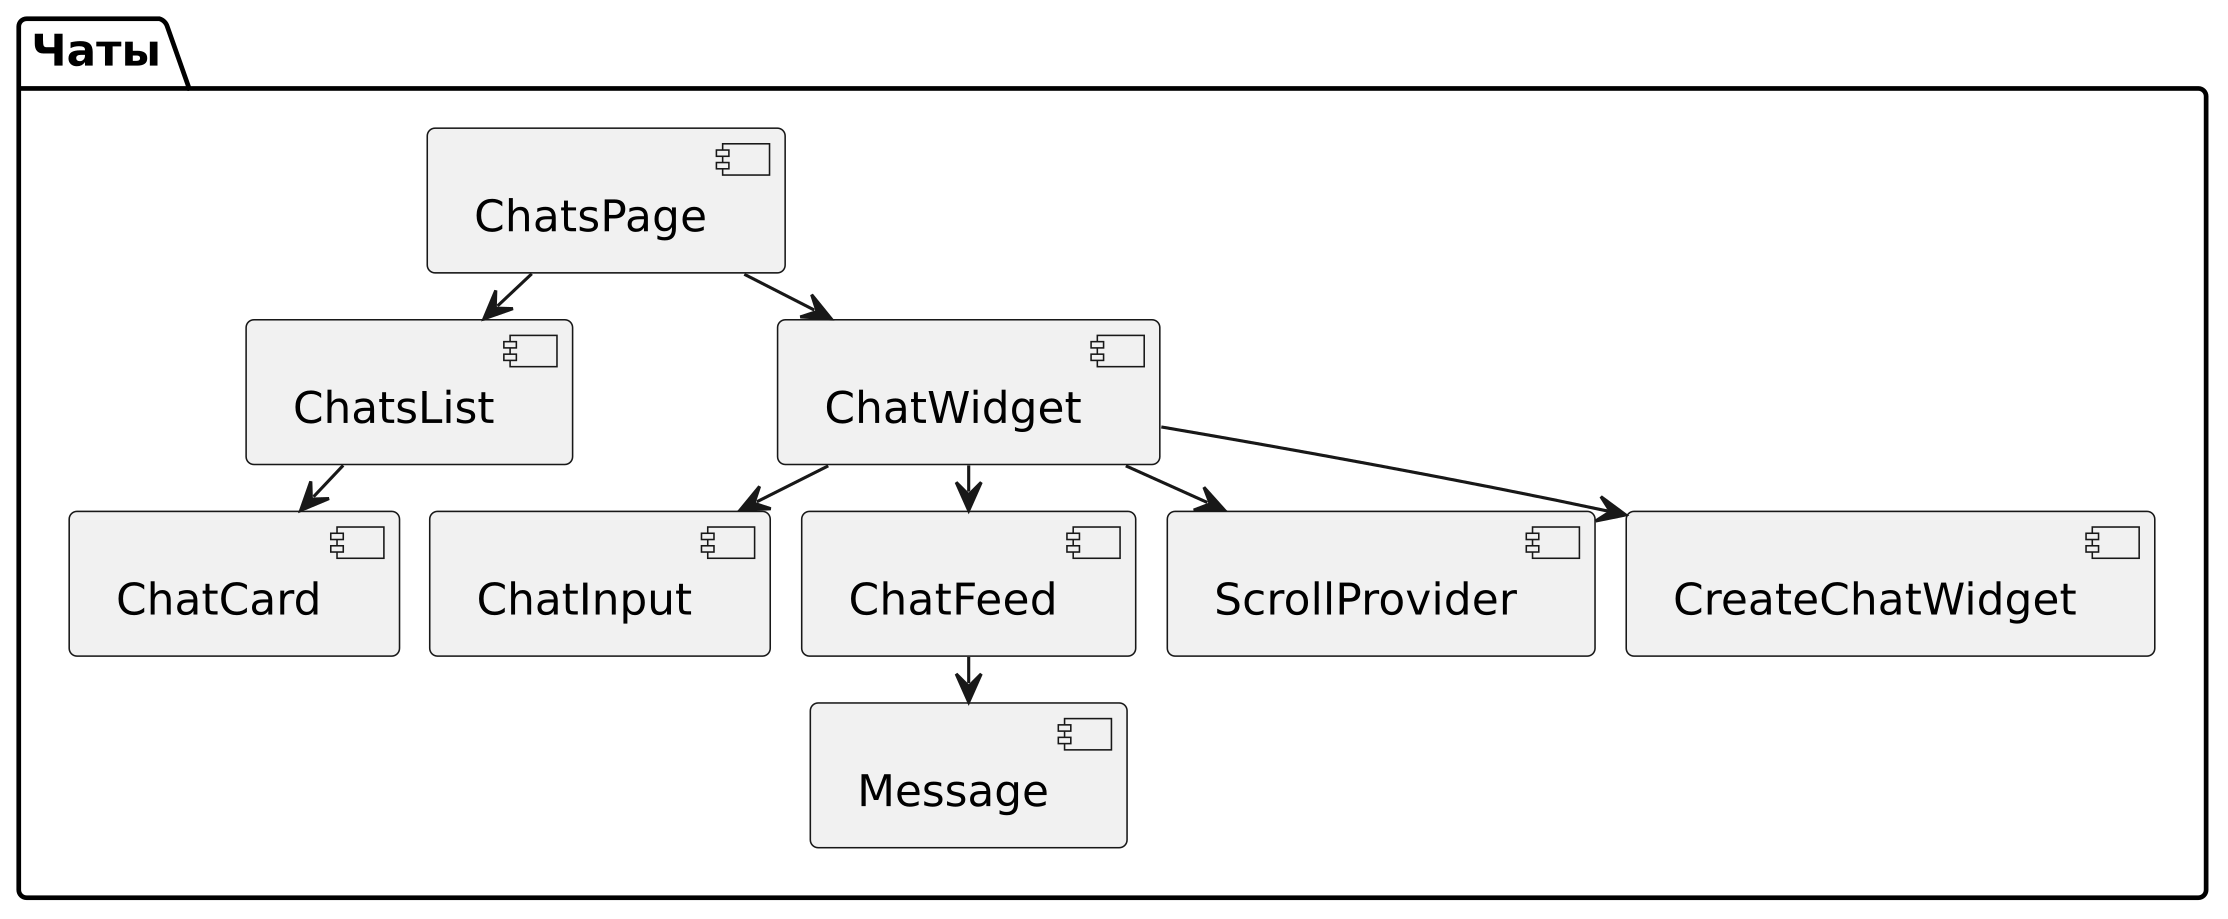
\includegraphics[width=0.9\textwidth]{static/diagrams/ChatsComponentDiagram.png}
\caption{Диаграмма компонентов системы чатов}
\label{fig:chat-components}
\end{figure}

Технически реализация основана на технологии WebSocket с использованием библиотеки \textit{Socket.IO}, что обеспечивает мгновенную доставку сообщений и минимальную задержку при передаче данных.

Основной функционал включает:
\begin{enumerate}
\item Подключение к соответствующим «комнатам» (группам или диалогам);
\item Отправку и приём текстовых сообщений;
\item Отображение истории переписки;
\item Поддержку вложений и индикаторов прочтения.
\end{enumerate}

Доступ к системе чатов осуществляется только после успешной авторизации, что исключает участие анонимных пользователей и обеспечивает безопасность переписки.

Подсистема анализа решений на основе искусственного интеллекта реализует автоматическую проверку студенческих заданий с использованием AI, что является одной из ключевых особенностей платформы.
Подсистема предназначена для получения и визуализации результатов анализа на основе искусственного интеллекта, включая оценку корректности текста программ, проверку на соответствие заданию, а также вывод комментариев, рекомендаций и текстовых пояснений.Результаты анализа отображаются в виде отчёта с возможностью преподавателя оставить дополнительные замечания. Таким образом, снижается нагрузка на преподавателя и повышается объективность оценивания.

Каждая из указанных подсистем обладает чётко определёнными входными и выходными данными, а также взаимодействует с другими модулями системы. Например, подсистема работы с заданиями напрямую связана с анализом на основе искусственного интеллекта, а система чатов — с механизмами авторизации и маршрутизации. Такое проектирование обеспечивает гибкость, надёжность и чёткую масштабируемость клиентской архитектуры.

\subsubsection{Страницы и их структура}

Разработка интерфейсной части веб-приложения требует не только реализации функциональных компонентов, но и проектирования логически связанных экранов, отражающих ключевые сценарии взаимодействия пользователя с системой. В рамках платформы каждая страница представляет собой самостоятельный интерфейсный модуль, обслуживающий одну или несколько бизнес-задач, соответствующих определённой роли: студент, преподаватель, администратор.

Процесс формирования страниц реализован с применением маршрутизации, встроенной в фреймворк \textit{Next.js}, что обеспечивает высокую производительность и поддержку серверного рендеринга. Страницы не только представляют визуальный уровень приложения, но и координируют работу между компонентами пользовательского интерфейса, бизнес-логикой и хранилищем состояния.

Архитектурно страницы собираются из обособленных функциональных элементов, разработанных согласно принципам FSD: пользовательские действия реализуются в слое \textit{features}, отображаемые сущности формируются на базе слоя \textit{entities}, а объединение этих блоков происходит внутри слоя \textit{widgets}. Такой подход позволяет повысить согласованность, переиспользуемость и модульность текст программ, а также снижает зависимость между различными частями интерфейса.

Далее описаны ключевые страницы, отражающие основную логику пользовательского взаимодействия.

Страница авторизации отвечает за вход пользователя в систему. Содержит форму для ввода учётных данных, а также реализует логику валидации, передачи данных на сервер, обработки ошибок и сохранения сессионного токена. После успешной авторизации пользователь перенаправляется на главную страницу, соответствующую его роли.

Страница заданий представляет собой ключевой интерфейс для организации и выполнения учебной деятельности. Интерфейс страницы включает:
\begin{enumerate}
\item Список классов и учебных групп, к которым привязан пользователь;
\item Перечень активных заданий в рамках каждой группы;
\item Доступ к подробному описанию заданий, срокам сдачи и параметрам оценивания;
\item Отправку решений и просмотр результатов, включая отчёты анализа на основе искусственного интеллекта.
\end{enumerate}
Для преподавателя дополнительно предоставляется интерфейс управления заданиями, а также доступа к аналитике по группам и студентам.

Административная панель института является основным рабочим инструментом пользователя с ролью администратора. Интерфейс включает:
\begin{enumerate}
\item Управление иерархией образовательного учреждения (институты, кафедры, группы);
\item Назначение и блокировка пользователей (студентов и преподавателей);
\item Просмотр структуры учреждения в табличной форме;
\item Генерацию и отправку приглашений на регистрацию;
\item Журнал событий и контроль активности пользователей.
\end{enumerate}
Все действия на данной странице требуют повышенного уровня доступа и сопровождаются системой уведомлений о результатах операций.

Страница чатов реализует коммуникационную составляющую платформы. Пользователь получает доступ к:
\begin{enumerate}
\item Перечню активных диалогов (личных и групповых);
\item Истории сообщений в рамках выбранного чата;
\item Форме для отправки сообщений и файлов;
\item Интерактивным элементам: индикаторы доставки, статус прочтения, поиск по переписке.
\end{enumerate}
Для преподавателей также предусмотрена возможность создания новых групповых чатов для своих учебных групп.

Все функциональные страницы приложения, за исключением экранов регистрации и входа, используют единый шаблон компоновки, обеспечивающий целостность визуального восприятия и унификацию пользовательского опыта. Данный шаблон включает в себя общие элементы интерфейса — верхнюю панель навигации, боковое меню и основной контейнер для отображения содержимого, который динамически наполняется в зависимости от текущего маршрута.

Использование общего каркаса позволяет сохранить структурную согласованность между различными разделами системы, облегчает адаптацию пользователей к интерфейсу и упрощает внедрение изменений. Кроме того, архитектурное разделение логики и представления на уровне страниц способствует инкапсуляции ответственности, а также повышает читаемость и сопровождаемость текста программ. В рамках маршрутизации обеспечивается централизованное управление доступом, фильтрацией и визуализацией данных с учётом ролей пользователей.

Таким образом, структура страниц приложения отражает как технические требования архитектуры, так и практическую ориентацию на удобство и эффективность работы конечных пользователей.

\subsubsection{Компоненты и принципы их структурирования}

Компонентная модель проекта выстроена на основе принципов повторного использования, инкапсуляции и чёткого разделения ответственности между уровнями абстракции. Все компоненты, применяемые в рамках клиентского интерфейса, условно делятся на два основных класса: общие (универсальные) и специфические (бизнес-ориентированные).

\begin{enumerate}
  \item Общие компоненты представляют собой переиспользуемые элементы пользовательского интерфейса, не зависящие от предметной области. К ним относятся кнопки, поля ввода, модальные окна, индикаторы загрузки, элементы навигации, уведомления и другие базовые визуальные элементы. Такие компоненты широко применяются на всех уровнях интерфейса и не содержат бизнес-логики.
  \item Специфические компоненты, разрабатываемые в слоях \textit{entities} и \textit{widgets}, предназначены для реализации прикладной логики и отображения конкретных сущностей системы. Примерами являются компоненты отображения сообщений в чате, карточек заданий, панели управления преподавателя, таблиц пользователей и др. Они обладают внутренним состоянием и часто включают обращение к хранилищу.
\end{enumerate}

Такое структурное разграничение существенно упрощает масштабирование проекта, облегчает поддержку и повторное использование элементов, а также способствует разделению труда между разработчиками.

\subsubsection{Распределение логики по слоям архитектуры}

Функциональная логика клиентской части системы строго распределяется по слоям архитектуры Feature-Sliced Design, что обеспечивает высокую модульность и инкапсуляцию поведения. Каждому слою соответствует свой уровень ответственности:

\begin{enumerate}
  	\item В слое \textit{entities} сосредоточена модель предметной области: типизация, структура сущностей, атомарные компоненты отображения, такие как \textit{Registration}, \textit{Department}, \textit{Group}. Данный слой реализует описание и базовое представление данных без привязки к конкретным действиям пользователя.
	\item Слой \textit{features} содержит реализацию отдельных действий, составляющих пользовательские сценарии: отправка сообщений, регистрация, загрузка задания, подтверждение действия и т.д. Эти модули инкапсулируют конкретные шаги взаимодействия пользователя с интерфейсом, часто включая локальное состояние. Функции из слоя \textit{features} могут быть использованы многократно и комбинироваться для построения более сложных сценариев.
	\item Слой \textit{widgets} представляет собой реализацию полноценных пользовательских сценариев — законченных интерфейсных блоков, решающих определённую задачу. Примеры: интерфейс чата, панель с заданиями, административный модуль управления группами. Каждый виджет объединяет несколько фич и сущностей, обеспечивая завершённую и логически связанную единицу поведения.
	\item Слой \textit{pages} выполняет роль точки входа и финальной сборки пользовательских сценариев. Здесь происходит выбор и компоновка виджетов в зависимости от маршрута, роли пользователя и контекста сессии. Кроме того, на уровне страниц задаются глобальные обёртки, обеспечиваются ограничения доступа, инициализируются загрузки данных и подключаются необходимые провайдеры. Таким образом, слой \textit{pages} являются связующим слоем между навигацией и пользовательским опытом.
\end{enumerate}

Такое строгое распределение обязанностей по слоям позволяет исключить дублирование логики, минимизировать связанность между модулями и обеспечить чёткую иерархию ответственности.

\subsubsection{Пользовательские сценарии}

Для повышения удобства и доступности платформы, особенно в условиях использования её разными категориями пользователей, были реализованы следующие решения в области пользовательского опыта:

\begin{enumerate}
  \item Централизованная навигация — через универсальный макет, включающий боковую и верхнюю панели, интерфейс остаётся единообразным и интуитивно понятным вне зависимости от текущего маршрута;
  \item Toast-уведомления — реализация мгновенной обратной связи при выполнении действий: успешная отправка формы, ошибка сети, получение новых сообщений;
  \item Обработка пустых состояний и ошибок — предусмотрены интерфейсы для ситуаций отсутствия данных, ошибок загрузки или недоступности сервера.
\end{enumerate}

В результате, пользователь получает предсказуемый и непрерывный опыт взаимодействия с системой вне зависимости от своей роли и уровня подготовки.

\subsubsection*{Вывод}

Проектирование интерфейсной части приложения основывается на чётком структурном и функциональном разграничении компонентов, ориентированном на принципы модульности и масштабируемости. Использование архитектуры Feature-Sliced Design позволяет изолировать бизнес-логику, визуальные компоненты и маршрутизацию, что делает интерфейс легко расширяемым и сопровождаемым.

Реализованная организация интерфейса, объединяющая единый шаблон компоновки, повторно используемые компоненты и специфические бизнес-модули, способствует формированию целостного пользовательского опыта. Выбранные решения обеспечивают удобство и логичность навигации, а также высокую отзывчивость системы при взаимодействии с пользователем.


Интерфейсная часть проекта построена на модульной архитектуре, основанной на бизнес-функциях. Подсистемы выделены логически, а их реализация изолирована в независимые модули, что повышает удобство поддержки, расширения и переиспользования компонентов.